%
%     ApJ article: Rapidly Rotating Suns and Active Nests of Convection
%
%     Benjamin Brown
%     JILA and Dept. Astrophysical & Planetary Sciences
%     UCB 440
%     University of Colorado
%     Boulder, CO   803090-0440
%
%     e-mail: bpbrown@solarz.colorado.edu
%
%     Written using using AASTex style sheets
%
%     Submitted April 30, 2008
%     Revision submitted July 1, 2008
%


%*********************************************************************%
%                                                                     %
%              Patchy Convection Section                              %
%                                                                     %
%*********************************************************************%
\chapter{Dynamics Within Confined Nests of Convection}
\label{chapter:active nests of convection}
The emergence of localized nests of convection at higher rotation
rates is a striking feature that calls out for an explanation.  In
many ways, it is quite surprising that convection chooses to be
confined to narrow intervals in longitude, but such states have also
been realized in a number of other dynamical systems.  Generally the
appearance of nests is a challenge to explain in detail, yet the onset
of spatially modulated states which are their precursor is better
understood. 

\label{sec:patches}
\section{Spatially Localized Convection in Other Settings}
The phenomena of spatially localized convection has a rich history,
variously appearing in laboratory experiments and numerical
simulations.  Much interest in confined states of convection was
motivated by the discovery of such states in binary fluid convection
\citep[e.g.,][]{ Anderson&Behringer_1990, Kolodner&Glazier_1990,
Niemela_et_al_1990, Surko_et_al_1991}, where traveling waves of
convection appear via subcritical Hopf bifurcations and near onset are
seen to evolve into traveling patches of convection separated by
regions of nearly quiescent fluid.  From a theoretical perspective,
these confined states near onset are accessible to weakly nonlinear
theory and considerable progress has been made in understanding their nature
\citep[e.g.,][]{Riecke_1992,Barten_et_al_1995b, Batiste_Knobloch_2005,
Batiste_et_al_2006, Burke_Knobloch_2007}.  The confined states found
in binary convection differ from our active nests of convection in
several respects.  The most important is that in binary convection
there is no net vertical transport of solute.  The confined states
instead pump solute horizontally and create regions of stable vertical
stratification in the quiescent regions.  A possibly related phenomena
is that of localized states in magnetoconvection, as studied by
\cite{Blanchflower_1999} and in 3-D by \cite{Blanchflower_Weiss_2002}.
Here single convective cells (called ``convectons'') formed in a
region of initially uniform strong vertical magnetic field by a process of
flux expulsion.  Convection within the localized states was strong and
was entirely suppressed in the surrounding medium.  These convectons could
contain several convective cells and were generally stationary, though
some solutions exhibited time dependent behavior.  Recently, progress
has been made addressing these systems in approximate 2-D models
\citep{Dawes_2007}.

Confined states are
also realized in other doubly diffusive systems, as in theoretical
studies of thermosolutal
convection \citep{Knobloch_et_al_1986, Deane_et_al_1987,
  Deane_et_al_1988, Spina_et_al_1998}.  In the latter studies a
variety of traveling convective patches were found, and in these
the convective transport of heat and solute was enhanced
compared to that in the interpatch regions.  In all cases the patches
propagated in the same direction as the individual convective cells,
though more slowly.  Such behavior persisted for long periods of time.  
These localized states occurred well above the onset of convection,
and convection continued in the interpatch regions.  There may also be
analogues in convection within the Earth's atmosphere, where
deep convection in the tropics tends to be organized on global scales
into regions of locally enhanced convection which propagate in a
prograde sense.  These organized convective structures are called the
Madden-Julien Oscillation and appear to have their origin in the
coupling of convective motions with equatorially trapped waves
 \citep[perhaps Rossby or Kelvin waves; see review by][]{Zhang_2005}.    



The spatially modulated states in our simulations of stellar
convection exist at Rayleigh numbers far above the onset of
convection.  Spatially modulated states in this parameter regime have
also been observed in geophysically motivated 3-D Boussinesq simulations of
convection within a thick, rotating spherical shell
\citep{Grote&Busse_2000, Busse_2002, Busse_Simitev_2005}. In these
studies, spatially localized states emerged at moderate Rayleigh
numbers, involving an equilibrium between the shearing flow of
differential rotation destroying convective eddies and the Reynolds
stresses in the convection driving the differential rotation.  These
effects led to localized states where convection occupied a limited
portion of the domain and the region outside the convective patch was
filled with quiescent streaming flow and almost no radial motions.  In
the quiescent regions the thermal gradients become increasingly
unstable until they are advected back into the patch where they help
sustain the convective eddies.  The patches in these geophysical
simulations moved slowly retrograde and persisted up to Rayleigh
numbers of about $10^6$.  Beyond this point the differential rotation
became so strong that no sustained convection was possible.  Instead
the system began to behave as a relaxation oscillator, with short
bursts of convection temporarily building a strong differential
rotation which then sheared out the convective eddies.  Convective
transport remained suppressed until the shear of differential rotation
decayed viscously, whereupon a new burst of convection would begin the
process anew.  In all cases with localized convection, significant
oscillations were seen in the kinetic energies of both differential
rotation and convection \citep{Grote&Busse_2000}.

 
Similar states have also been realized in anelastic simulations of
stellar convection in spherical shells for a rotating younger sun with
a much thicker convection zone
\citep{Ballot_et_al_2006,Ballot_et_al_2007}.  The spatially modulated
states found there appear in the equatorial convection for models with
low Prandtl number ($\mathrm{Pr}=0.25$, as in the models of this paper).
Localized states turn into bursty, vacillating convection at large
Taylor numbers ($\mathrm{Ta} \gtrsim 10^9$), much like those in
\cite{Grote&Busse_2000}.  Localized states observed in thick
convective shells (with typical aspect ratios $\chi =
r_\mathrm{bot}/r_\mathrm{top}=0.58$) differ in many important respects
from the states we find in our relatively thin shells of convection
($\chi = 0.76$), most notably in their temporal stability, which we
will next discuss.

\section{Properties of the Active Nests}
Our active nests of convection appear first as regions of mildly
enhanced convective amplitude.  As the rotation rate increases, convection
in the equatorial regions gradually becomes more localized (as in Fig.~\ref{fig:ab2_turf}) and eventually is
present only within the active nest.  In some of our systems we observe two
nests or patches in longitude (such as case~G5) and in some only a
single nest (as in case~G10).  Generally,
convection at the highest rotation rates possesses only a single nest, and
for moderate rotation rates the system can alternate between two-nest
states and single-nest states, suggesting that several attractors
exist within the phase space.

To study the temporal evolution of our convective patterns in more
detail, we employ time-longitude maps as shown in
Figure~\ref{fig:time_longitude_map_turf5_all_3_depths}.  Here radial
velocities are sampled at the equator for all longitudes, considering
case~G5 at three depths (near the top, middle and bottom of the
convection zone) and doing so over an interval of 260 days (or about
45 rotation periods).  In these maps, structures propagating in a
prograde fashion relative to the frame of reference are tilted to the
upper-right and patterns propagating in a retrograde sense tilt to the
upper-left.  To construct these maps we have chosen a frame of
reference propagating in a prograde sense relative to the bulk
rotation frame ($\Omega_0=1.3 \times 10^{-5}~\mathrm{rad}~\mathrm{s}^{-1}$ 
or 2070~nHz), with constant relative angular velocity 
$6.75 \times 10^{-7}~\mathrm{rad}~\mathrm{s}^{-1}$
(107~nHz, for a total rotation rate of $1.052~\Omega_0$).  This
corresponds to the propagation rate of the modulated convection
pattern, and thus the nests appear stationary in this frame.  In the
$\Omega_0$ reference frame the nest takes about 108~days to complete
one lap around the equator, thus for the time interval shown in
Figure~\ref{fig:time_longitude_map_turf5_all_3_depths} the nests
travel about $870^\circ$ in longitude and completes about 2.4 circuits
around the equator. The active nests of convection can persist for
extremely long periods of time.  The two nests visible in
Figure~\ref{fig:time_longitude_map_turf5_all_3_depths} remain
coherent for over 5000 days of simulated time.

%%%%%%%%%%%%%%%%%%%%%%%%%%%%%%%%%%%%%%%%%%%%%%%%%%%%%%%%%%%%%%%%%%%%%%%%%%%%%%%%%%%%%%%%%%
\begin{figure*}
  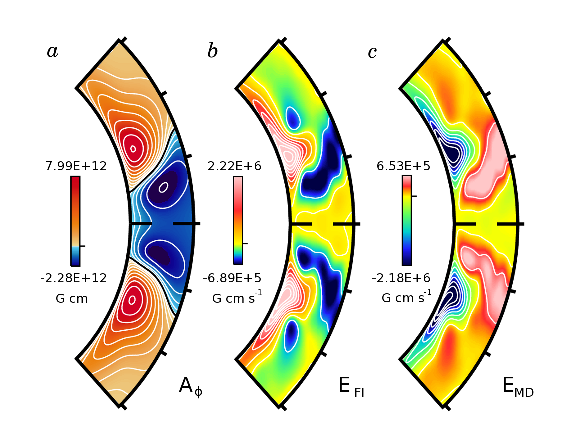
\includegraphics[width=\linewidth]{figs/chapter_4/Figure_14.eps}
  %\plotone{f14.eps}
  \caption[Nests of convection in G5 shown in time-longitude maps at three depths]
  {Nests of convection in G5 shown in time-longitude maps at three
  depths. Radial velocity $v_r$ is sampled ($a$)~near top
  ($0.95\thinspace R_\odot$), ($b$)~middle ($0.85\thinspace R_\odot$)
  and ($c$)~bottom ($0.73\thinspace R_\odot$) of layer.
  These samples are extracted at the equator, using a reference frame
  tracking the nests and starting from a mature state in the simulation.
  Two nests are visible, and individual convective cells appear
  as paired upflows and downflows, which propagate slightly faster than the mean zonal flow that they
  establish and thus pass through the nests.
  ($d,e,f$) Time averages with longitude of entropy fluctuations
  $\widetilde{S}$ and convective kinetic energy density $\widetilde{K}$ in these samples.
  \label{fig:time_longitude_map_turf5_all_3_depths}}
\end{figure*}
%%%%%%%%%%%%%%%%%%%%%%%%%%%%%%%%%%%%%%%%%%%%%%%%%%%%%%%%%%%%%%%%%%%%%%%%%%%%%%%%%%%%%%%%%%

Individual convective upflows and downflows appear as streaked red and blue regions
respectively.  In the upper convection zone ($0.95 R_\sol$), the
convective cells propagate more rapidly than the nests of convection.
Here they overtake the nests from behind (from smaller longitudes) and
then slowly swim through at a reduced speed.  Within the nests
convective cells collide and interact, and the strongest survive to
emerge from the front of the nest, where they speed up as they then
propagate through the more quiescent region.  
When this occurs, typically a small wave train comprised of 2 to 3
upflow/downflow pairs escapes, and as they enter the quiescent regions
these convective cells speed up to once again outpace the zonal flow.
In the lower convection
zone ($0.73 R_\sol$), the nests propagate more rapidly than the
convective cells, and the individual upflows and downflows appear as
strong retrograde-directed streaks.  Also visible in the lower
convection zone are low-amplitude velocity structures of rapid retrograde
propagation.  They appear to be the weak
equatorward extension of the large-scale (retrograde rotating) polar
patterns evident in Figure~\ref{fig:G5_thermal_structure}.  At
mid-convection zone ($0.85 R_\sol$), nearly all vertical flow is
occurring within the nests of active convection, though the strongest
cells outside the nest in the upper convection zone manage to weakly
print down to this intermediate depth.

 
The typical angular velocities of the differential rotation, the
individual convective cells and the active nests of convection are
shown in Figure~\ref{fig:patch_velocity_cartoon} for case~G5 and
detailed for several cases in Table~\ref{table:angular velocities}.  The nests of
convection propagate at a constant angular velocity at all depths in
the convection zone and over the entire range of latitudes ($\pm
30^\circ$) where they are present.  In contrast, the angular velocity $\Omega$
of the differential rotation varies substantially with radius and
latitude.  At all depths, the individual convective cells propagate
more rapidly than the zonal flow of differential rotation which they drive.  Because
the nests of convection propagate at an intermediate prograde rate,
they experience a head-wind from the differential rotation in the deep
convection zone and a tail-wind near the
surface.  Despite this strong radial shear, the
nests remain coherent across the entire convection zone for long
periods compared with either the lifetime of individual convective
cells (10-30 days), the rotation period of the star (5 days) or
typical thermal and viscous diffusion times ($\tau_\kappa =
910~\mathrm{days}$, $\tau_\nu=3640~\mathrm{days}$, both at mid-depth).
The time for the differential rotation to lap the nests at the
equator is about 112 days near the surface and 143 days at the bottom of the shell.

%%%%%%%%%%%%%%%%%%%%%%%%%%%%%%%%%%%%%%%%%%%%%%%%%%%%%%%%%%%%%%%%%%%%%%%
\begin{figure}[!tp]
  \begin{center}
    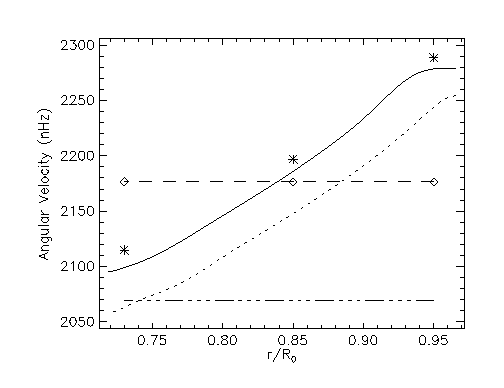
\includegraphics[width=0.7\linewidth]{figs/chapter_4/Figure_15.eps}
  \end{center}
  %\plotone{f15.eps}
  \caption[Angular velocities of various structures with radius in case~G5]
          {Angular velocities of various structures with radius in case~G5.  
  The mean shearing zonal flow of differential rotation $\Omega$ is denoted for all
  depths at the equator (solid curve) and at $\pm
  15^\circ$ latitude (dotted).  The propagation rate of the
  active nests (diamonds) is constant across the 
  entire latitude and radial range where they appear ($\pm 30^\circ$).
  The average velocity of individual convective cells at the equator
  (asterisks) is more rapid than the mean zonal flow they
  establish.  Their propagation is faster than the nests
  near the top and slower near the bottom.
  The global rotation rate $\Omega_0$ is 2070 nHz (marked). 
  \label{fig:patch_velocity_cartoon}}
\end{figure}
%%%%%%%%%%%%%%%%%%%%%%%%%%%%%%%%%%%%%%%%%%%%%%%%%%%%%%%%%%%%%%%%%%%%%%%
 

 
%%%%%%%%%%%%%%%%%%%%%%%%%%%%%%%%%%%%%%%%%%%%%%%%%%%%%%%%%%%%%%%%%%%%%%%%%%%%%%%%%%%%%%%%%%
\begin{deluxetable}{lcccccc}
\tablecaption{Angular Velocities of Various Structures\label{table:angular velocities}}
\tablewidth{0pt}  % `natural' size
\tablehead{\colhead{Case} 
& \colhead{$\Omega_0$}
& \colhead{$\Omega_\mathrm{nest}$}
& \colhead{$\Omega_{\mathrm{eq},\mathrm{top}}$}
& \colhead{$\Omega_{\mathrm{eq},\mathrm{bot}}$}
& \colhead{$\Omega_{c,\mathrm{top}}$}
& \colhead{$\Omega_{c,\mathrm{bot}}$}
}
\startdata
G1  & \phn2.60 & ---   & 0.341 & 0.060 & 0.535 & 0.180 \\
G3  & \phn7.80 & 0.511 & 1.094 & 0.220 & 1.176 & 0.330 \\ 
G5  & 13.00    & 0.675 & 1.319 & 0.197 & 1.381 & 0.288 \\ 
G10 & 26.00    & 0.830 & 1.497 & 0.140 & 1.623 & 0.280 \\[0.25cm]  

G3a & \phn7.80 & 0.690 & 1.295 & 0.265 & 1.421 & 0.373 \\ 
G3b & 13.00    & 0.670 & 1.555 & 0.250 & 1.590 & 0.413 \\
G5b & 13.00    & 0.750 & 1.778 & 0.246 & 1.800 & 0.430 \\[0.1cm]
\enddata
\tablecomments{All angular velocities in
  $\mu\mathrm{rad}\thinspace\mathrm{s}^{-1}$ and, except for the frame
  rate $\Omega_0$, are given relative to $\Omega_0$.
  The differential rotation at the equator $\Omega_\mathrm{eq}$ is measured at
  $0.95R_\sol$ (\emph{top}) and $0.73R_\sol$ (\emph{bot}).   The mean propagation rate of
  individual convective structures $\Omega_c$ is measured at the same
  depths in time-longitude maps of $v_r$ and has a typical variance of 
  $\pm 0.04~\mu\mathrm{rad}\thinspace\mathrm{s}^{-1}$ .} 
\end{deluxetable}
%%%%%%%%%%%%%%%%%%%%%%%%%%%%%%%%%%%%%%%%%%%%%%%%%%%%%%%%%%%%%%%%%%%%%%%%%%%%%%%%%%%%%%%%%%
 



%%%%%%%%%%%%%%%%%%%%%%%%%%%%%%%%%%%%%%%%%%%%%%%%%%%%%%%%%%%%%%%%%%%%%%%%%%%%%%%%%%%%%%%%%%
\begin{figure}
  \begin{center}
    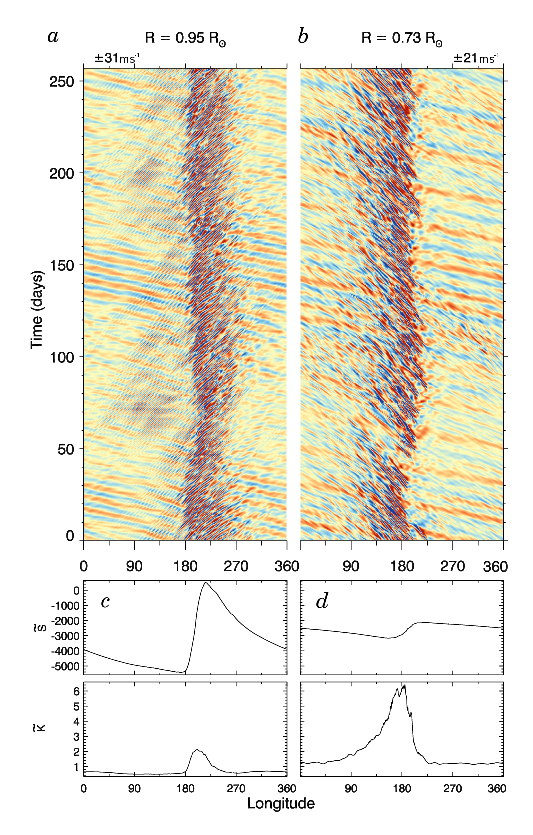
\includegraphics[width=0.7\linewidth]{figs/chapter_4/Figure_16.eps}
  \end{center}
  %\plotone{f16.eps}
  \caption[Time-longitude map of single nest of convection in case~G10]
  {Time-longitude map of single nest of convection in case~G10.
    As in Fig.~\ref{fig:time_longitude_map_turf5_all_3_depths},
    radial velocity $v_r$ is shown ($a$)~near top and ($b$)~near bottom of layer.
    Here a single nest is realized, with individual
    convective cells almost entirely confined to the nest, though they
    continue to propagate within it.
    ($c,d$)~Time averages $\widetilde{S}$ and $\widetilde{K}$ constructed in the
    same reference frame.
  \label{fig:time_longitude_map_turf10_2_depths}}
\end{figure}
%%%%%%%%%%%%%%%%%%%%%%%%%%%%%%%%%%%%%%%%%%%%%%%%%%%%%%%%%%%%%%%%%%%%%%%%%%%%%%%%%%%%%%%%%%
 

At the higher rotation rates, single stable nests of convection
dominate the equatorial region.  Time-longitude maps are shown in
Figure~\ref{fig:time_longitude_map_turf10_2_depths} for the equatorial
radial velocity at two depths in case~G10, our most rapidly rotating simulation.
Within the nest, convection remains vigorous, with the strongest
downflow networks still spanning the entire depth of the convection
zone.  This nest again propagates in a prograde sense relative to
$\Omega_0$, with constant relative angular velocity $8.3\times
10^{-7}~\mathrm{rad}~\mathrm{s}^{-1}$ (132~nHz, for a total rotation
rate of $1.032~\Omega_0$).  Over the interval shown the nest completes
almost 3 circuits of the equator relative to the $\Omega_0$ reference
frame.  Individual convective cells continue to swim through the nest,
moving more rapidly near the surface and more slowly in the deep
convection zone.  The very strong radial shear prevents all but the
strongest of downflows from spanning the full convection zone.  In the
region outside the nest, convection is strongly suppressed and the
main features are the weak flows associated with the retrograde
propagating polar pattern.  In the upper convection zone, occasional
weak convective disturbances appear upstream of the nest.  As these
fluctuations enter the nest they grow in amplitude.

 
Our nests of active convection may owe their existence to a
competition between the shearing action of differential rotation
acting on the individual convective eddies and Reynolds stresses
within the convection helping to maintain the strong zonal flows.  Unlike
the systems studied by \cite{Grote&Busse_2000} and
\cite{Ballot_et_al_2007}, our patchy convection is not accompanied by
relaxation oscillation behavior or large exchanges between the kinetic
energy in convection and in the differential rotation.  Rather, our
nests are not bursty in time and instead persist for long periods in
quasi-steady states.  This is true even for our most rapidly rotating
case considered here (G10) and at much higher turbulent
driving (G5b), though these simulations exist at Taylor
numbers below the threshold suggested by \cite{Ballot_et_al_2007}
($\mathrm{Ta} \gtrsim 10^9$).  Coupling between equatorially trapped waves and
convection may also have a role, but the contribution
of this coupling to spatial localization has been difficult to elucidate.


\section{Detailed Structure of an Active Nest of Convection}

 
%%%%%%%%%%%%%%%%%%%%%%%%%%%%%%%%%%%%%%%%%%%%%%%%%%%%%%%%%%%%%%%%%%%%%%%%%%%%%%%%%%%%%%%%%%
\begin{figure}
  \begin{center}
    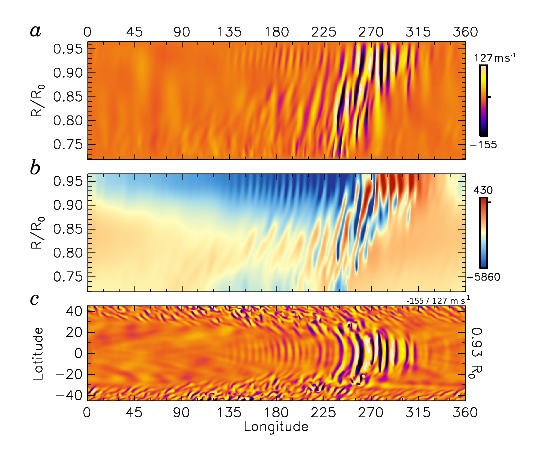
\includegraphics[width=0.9\linewidth]{figs/chapter_4/Figure_17.eps}
  \end{center}
  %\plotone{f17.eps}
  \caption[Detailed structure of convective nest in case~G10]
   {Detailed structure of convective nest in case~G10.  This snapshot
   of nest structure is shown at relative day 221 of
    Fig.~\ref{fig:time_longitude_map_turf10_2_depths}.  ($a$)~Radial
    velocities in an equatorial cut shown for all longitudes and
    radii.  
    ($b$)~Companion entropy fluctuations $S$ about
    their spherical means $\bar{S}$ (in cgs units), with high entropy
    fluid in red tones.
    ($c$)~Radial velocity in the equatorial region shown near the top of layer.
    \label{fig:G10_patch}}
\end{figure}
%%%%%%%%%%%%%%%%%%%%%%%%%%%%%%%%%%%%%%%%%%%%%%%%%%%%%%%%%%%%%%%%%%%%%%%%%%%%%%%%%%%%%%%%%%
 

We focus here on the structure of the nests so evident in
Figures~\ref{fig:time_longitude_map_turf5_all_3_depths} and
\ref{fig:time_longitude_map_turf10_2_depths} for cases~G5 and~G10, but
devote particular attention to the single nest realized in the latter
as a representative case.  The active nests extend throughout the
depth of the convection zone.  This is illustrated most clearly in
Figure~\ref{fig:G10_patch}$a$, showing the vertical profile
of radial velocities with longitude in a cut at the equator.
Convection is broken into multiple cells, one set above $0.9 R_\sol$
and another below $0.8 R_\sol$.  Only within the nest do strong downflows
span the convection zone.  The nest is embedded in a region of strong
latitudinal and radial zonal shear (as shown by the tilted nature of
its structure), yet the pattern propagates at a constant angular
velocity at all depths and latitudes.  At the surface and near the
equator the nest propagates more slowly than the zonal wind,
whereas at the base of the convection zone it propagates more rapidly.
Individual convective structures swim still more rapidly and both
enter and exit the region of enhanced convection.  As such, the nest
experiences a strong retrograde flow at the base and a strong prograde
flow near the surface.  

The thermal structure of the nests is revealed by their entropy
fluctuations, as shown in Figure~\ref{fig:G10_patch}$b$.  In the upper
convection zone, the mean zonal flow advects low entropy fluid into
the nests from the left side.  This fluid is then swept away by
intermittent downflows and replaced by higher
entropy fluid from below.  In the lower convection zone, higher entropy
fluid is swept into the nest from the right and lower entropy exits to
the left.  At mid convection zone, regions outside the nest remain
convectively unstable, but only weak radial motions are driven here.


 
%%%%%%%%%%%%%%%%%%%%%%%%%%%%%%%%%%%%%%%%%%%%%%%%%%%%%%%%%%%%%%%%%%%%%%%%%%%%%%%%%%%%%%%%%%
\begin{figure}
  \begin{center}
    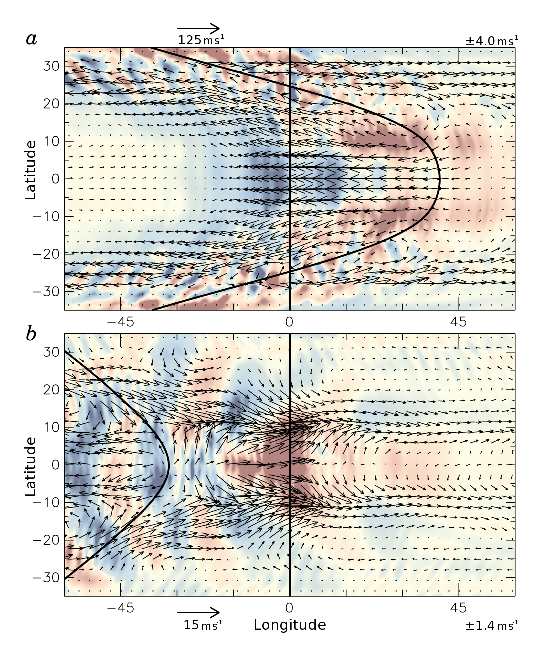
\includegraphics[width=0.8\linewidth]{figs/chapter_4/Figure_18.eps}
  \end{center}
  %\plotone{f18.eps}
  \caption[Mean circulations associated with the nest in case~G10]
          {Mean circulations associated with the nest in case~G10.  
  ($a$) Time averaged radial (colors) and horizontal flows (arrows)
  near the top and ($b$) near the bottom of the shell, in a reference
  frame tracking the nest.  The strong zonal flow of differential rotation has
  been subtracted at each latitude and 
  is shown by the solid curves (both scaled by
  $125~\ms$ arrow length, with zero velocity relative to the
  nest indicated by the vertical line).
  Within the nest strong eddy currents partially decelerate
  the flow, while outside the streaming mean zonal flow dominates. 
  \label{fig:G10_tracked_nest}}
\end{figure}
%%%%%%%%%%%%%%%%%%%%%%%%%%%%%%%%%%%%%%%%%%%%%%%%%%%%%%%%%%%%%%%%%%%%%%%%%%%%%%%%%%%%%%%%%%
 

The mean longitudinal structure of the nests can be assessed by
forming temporal averages of various properties in a frame co-rotating
with the nests of convection (these averages denoted by a tilde).
This is done at the equator for entropy $\widetilde{S}$ and 
convective kinetic energy density $\widetilde{K}$ (with same form as CKE) 
for case~G5 in Figure~\ref{fig:time_longitude_map_turf5_all_3_depths}$d-f$ and for 
case~G10 in Figure~\ref{fig:time_longitude_map_turf10_2_depths}$c,d$.
There are distinctive differences between the leading (to the right)
and trailing (to the left) portions of the profiles, with $\widetilde{S}$ showing
a gradual rise and steeper drop in going to decreasing longitudes
(from right to left).  The envelope of $\widetilde{S}$ is largely similar in form
at the top and bottom of the convection zone.  In contrast $\widetilde{K}$,
which traces the fluctuating velocities of convection, changes form
with depth, being skewed in the direction of the mean zonal flow.  At
the top of the convection zone this sense of skew is toward the
right, and at the bottom it is toward the left.

These nests must have gradual circulations associated with them, though these
are a challenge to discern as they are much weaker than the strong
mean zonal flows.  We can get some sense of them by averaging the
vertical and horizontal flows in the surroundings of a nest while
tracking it over long time intervals.  Shown in
Figure~\ref{fig:G10_tracked_nest} are the slow circulations associated
with the nest in case~G10 near the top and bottom of the convection zone.  
These flows have been averaged over a period of 615~days starting
at the beginning of the interval shown in
Figure~\ref{fig:time_longitude_map_turf10_2_depths}.  
The flows suggest a systematic zonal circulation from fore to aft in the upper
convection zone and toward higher latitudes and diverging from the nest
at depth, though to achieve this we have subtracted the fast mean
zonal flow which varies with latitude as shown.  
The mean upflows and downflows in the nest are quite weak, with amplitudes
of a few $\ms$, as compared with the convection which can have
peak velocities of a few hundred $\ms$.
Test particles released in the flow would not simply circulate
according to these mean circulations and would
be instead swept along by the strong mean zonal flow and of course by
the vigorous convection cells that propagate through the nest.  Some
test particles would encounter strong downflows and would be swept
down through the nest to the bottom of the convection zone while
others would likely be carried horizontally out the nest and remain at
a similar depth.
Yet Figure~\ref{fig:G10_tracked_nest} indicates that a weak large-scale
circulation is realized, and this may serve to slowly pump fluid
through the system.  These mean circulatory flows may also serve to inform
analytic models of such nests of convection.



%*********************************************************************%
%                                                                     %
%              Conclusions                                            %
%                                                                     %
%*********************************************************************%

\clearpage
\section{Conclusions}
\label{sec:nests conclusion}
A striking feature of these simulations is the emergence of a 
pattern of strongly modulated convection in the equatorial regions.  These
nests of active convection are regions of enhanced convective vigor
and transport which propagate at rates distinct from either the mean
zonal flows of differential rotation or the individual convective
cells.  In the most rapidly rotating systems, such as case~G10,
convection at the equator is entirely dominated by motions inside the
nest with only very weak radial motions present in the regions
outside the nest.  Though their impact on the convection is most
obvious in the rapidly rotating limit, we find some evidence for weak
modulation even in our more slowly rotating cases.

All of our simulations stop short of the turbulent stellar surface,
and it is thus difficult to estimate how these nests of active
convection may affect stellar observations in detail.  The convective velocities
associated with the nests are small compared to the nearly supersonic
flows in stellar granulation, and in the Sun such global-scale
convective structures have evaded direct detection despite intensive
searches throughout the near-surface layers by helioseismology.  The
extremely localized nests found in our most rapidly rotating cases may
however influence the thermal stratification and thus convective vigor
in the near surface regions, as most of the flux at the equator is
transported through a narrow range of longitudes.  These nests may act
as traveling hot spots with enhanced convection even in the surface
layers where the higher emerging flux escapes the system.

These spatially localized states of convection may also have some bearing
on the active longitudes of magnetic activity observed in the Sun, if
the enhanced pummeling of the tachocline by the convection within the
nest preferentially destabilizes magnetic structures within the
tachocline that then rise to the surface.  
If they do survive in a magnetic environment, then their strongest signature is
likely to emerge in magnetic stars, where magnetic fields threading
the bulk of the convection zone may be concentrated in the nests and 
mimic giant, propagating starspots which survive for very long epochs
in time.  If the nests lead to active
longitudes of enhanced magnetic activity in rapidly rotating stars, we
might expect these long-lived magnetic structures to propagate at a
rate different from the stellar rotation rate as measured at the
surface or from the stellar differential rotation.

We recognize that our simulations remain separated
by many orders of magnitude from the parameter space of real stellar
convection.  As such, we must be cautious with our interpretations of
the overall dynamics.  However, we have found that these nests of
convection are a robust feature over a range of parameters and that
they are able to persist as entities for as long as we could pursue their
modelling.  Thus one should be prepared to consider the possibility of
their presence also in real stellar convection zones, where they may
appear as long-lived propagating features.


Our current family of dynamo simulations indicate that nests of
convection can coexist with magnetism in portions of parameter space.
We will explore this possibility in 
Chapter~\ref{chapter:menagerie of dynamos}, but first we turn to a
more general exploration of dynamo activity in these rapidly rotating suns.


